%%%%%%%%%%%%%%%%%%%%%%%%%%%%%%%%%%%%%%%%%%%%%%%%%%%%%%%%%%%%%%%%%%%%%%%%%%%%
\section{General version control concepts}

\begin{frame}{What is version control?}

\begin{description}
\item[Administrator] Organises and takes care of the history and different
    versions, trees and flows in a project (e.g. software development,
    document writing, server administration).
\item[Time machine] One can see and reinstate old states of files and entire
    projects.
\item[Quasi-backup] When the repository is kept on a separate server then
    this is basically a backup of the project.
\end{description}

\end{frame}


%%%%%%%%%%%%%%%%%%%%%%%%%%%%%%%%%%%%%%%%%%%%%%%%%%%%%%%%%%%%%%%%%%%%%%%%%%%%
\begin{frame}
\frametitle{Using version control}
{\large \alert{Who uses version control?}}

Everyone who would like to access an old version of a document.  Or everyone
to whom such things have happened:
\begin{itemize}
    \item \enquote{It would be nice to have the version from 2 hours ago \ldots}
    \item \enquote{I wrote that really well three days ago.  How did that go
        again?}
    \item \enquote{Oh no!  I deleted the file!}
\end{itemize}

{\large \alert{Where is version control used?}}
\begin{itemize}
\item Software development
\item Text and document processing/writing
\item Graphic design
\item System administration
\end{itemize}
\end{frame}

%%%%%%%%%%%%%%%%%%%%%%%%%%%%%%%%%%%%%%%%%%%%%%%%%%%%%%%%%%%%%%%%%%%%%%%%%%%%
\begin{frame}
\frametitle{Using version control (cont.)}
{\large \alert{What kinds of files should be kept under version control?}}

\begin{itemize}
\item Any kind of file which will be changed
\item Mainly text files
    \begin{itemize}
    \item Program code
    \item Documentation
    \item Theses, Dissertations
    \end{itemize}
\item But also binary files
    \begin{itemize}
    \item Graphics files; \ttalert{.png}, \ttalert{.tiff}
    \item Documents; \ttalert{.pdf}, \ttalert{.odt}
    \end{itemize}
\end{itemize}

{\large \alert{What shouldn't be kept under version control?}}

\begin{itemize}
\item Automatically generated files, e.g.: \ttalert{.o}, \ttalert{.log},
    \ttalert{.pdf}
\item Editor \enquote{backup} files, e.g.: \ttalert{file\~}, \ttalert{file.bak}
\end{itemize}

\end{frame}


%%%%%%%%%%%%%%%%%%%%%%%%%%%%%%%%%%%%%%%%%%%%%%%%%%%%%%%%%%%%%%%%%%%%%%%%%%%%
\begin{frame}[fragile]
\frametitle{Version control systems}
{\large \alert{Versions in file names}}

Does this look familiar?
\begin{lstlisting}
$ ls
file.1  file.20090803  file.keep  file.new  file.old.2
file.2  file.alt       file.neu   file.old
\end{lstlisting}

This is better than nothing, however what happened between the different
versions?  Which file is actually the most current?

{\large \alert{Automatic version control}}

There are many programs which can be used for the administration and
organisation of files:

\begin{itemize}
\item SCCS, RCS, CVS, Subversion, Git, Mecurial, Arch, Darcs, \ldots
\end{itemize}

\end{frame}


%%%%%%%%%%%%%%%%%%%%%%%%%%%%%%%%%%%%%%%%%%%%%%%%%%%%%%%%%%%%%%%%%%%%%%%%%%%%
\begin{frame}{Editing models}

\begin{itemize}
\item lock-modify-unlock  (RCS, also CVS, Subversion)
    \begin{itemize}
    \item File is checked out and locked; it can only be changed by one user
    \item File is modified
    \item File is checked in and unlocked
    \item \tbf{Disadvantage:} very inflexible
    \item \tbf{Advantage:} reduced effort when editing graphics files
    \end{itemize}
\item copy-modify-merge (CVS, Subversion, Git, \ldots)
    \begin{itemize}
    \item All files are copied from the repository and can be modified
        without restriction and independently of other copies
    \item When checking in modifications, the changes are automatically
        merged with other changes
    \item \tbf{Disadvantage:} Conflicts between changes can occur
    \item \tbf{Advantages:} very flexible; several people can work at the
        same time
    \end{itemize}
\end{itemize}

\end{frame}


%%%%%%%%%%%%%%%%%%%%%%%%%%%%%%%%%%%%%%%%%%%%%%%%%%%%%%%%%%%%%%%%%%%%%%%%%%%%
\begin{frame}{Repository models}

\begin{itemize}
\item Centralised Repository Model (client-server)
\end{itemize}
\begin{center}
    \resizebox{!}{0.7\textheight}{
        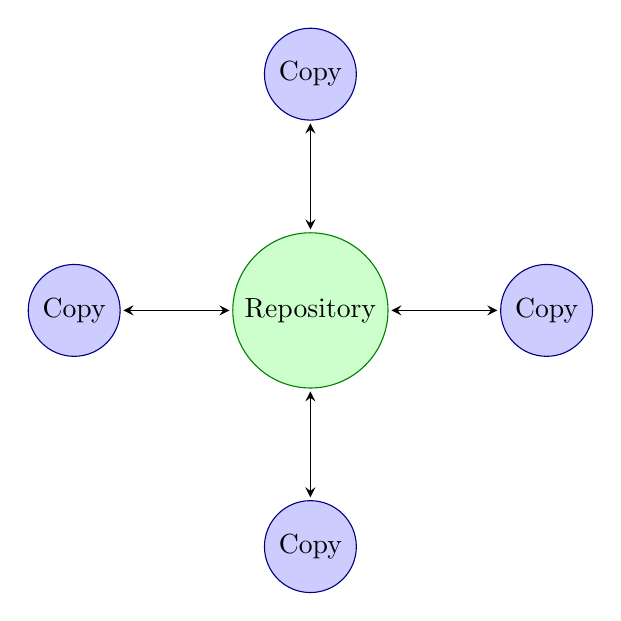
\begin{tikzpicture}
[repo/.style={circle,
		fill=green!20!white,
		draw=green!50!black,
		minimum size=10mm},
workingcopy/.style={circle,
		fill=blue!20!white,
		draw=blue!50!black,
		minimum size=5mm},
link/.style={<->, shorten <=1pt, shorten >=1pt, >=stealth, semithick}]

% central repo
\node at (0, 0) [repo] (mainrepo) { Repository };
% working copies
\node at (3,0)  [workingcopy] (copyright)  { Copy };
\node at (-3,0) [workingcopy] (copyleft)   { Copy };
\node at (0,3)  [workingcopy] (copytop)    { Copy };
\node at (0,-3) [workingcopy] (copybottom) { Copy };
% links between repo and working copies
\draw [link] (mainrepo) -- (copyright);
\draw [link] (mainrepo) -- (copyleft);
\draw [link] (mainrepo) -- (copytop);
\draw [link] (mainrepo) -- (copybottom);
\end{tikzpicture}

    }
\end{center}

\end{frame}

%%%%%%%%%%%%%%%%%%%%%%%%%%%%%%%%%%%%%%%%%%%%%%%%%%%%%%%%%%%%%%%%%%%%%%%%%%%%
\begin{frame}{Repository models (cont.)}

\begin{itemize}
\item Distributed Repository Model (pure); e.g. Linux Kernel
\end{itemize}
\begin{center}
    \resizebox{!}{0.7\textheight}{
        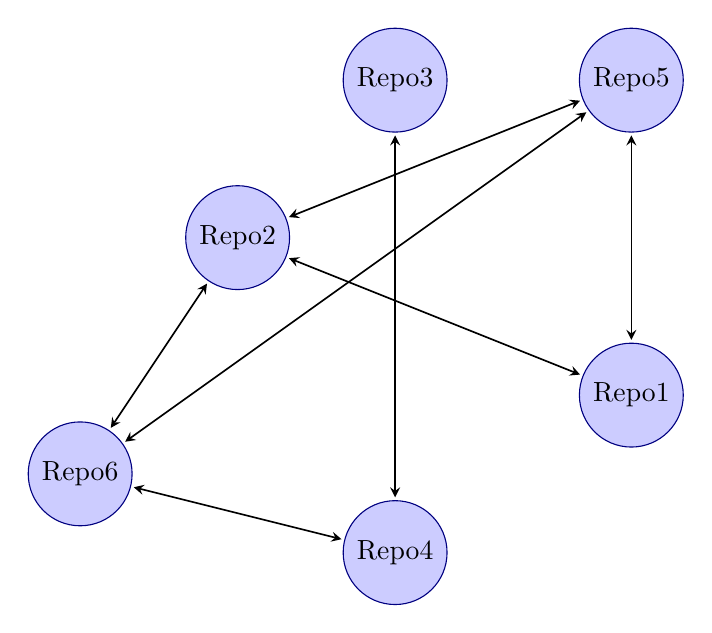
\begin{tikzpicture}
[repo/.style={circle,
		fill=green!20!white,
		draw=green!50!black,
		minimum size=10mm},
workingcopy/.style={circle,
		fill=blue!20!white,
		draw=blue!50!black,
		minimum size=5mm},
link/.style={<->, shorten <=1pt, shorten >=1pt, >=stealth, semithick}]

% central repo
%\node at (0, 0) [repo] (mainrepo) { Repository };
% working copies
\node at (3,-1)  [workingcopy] (repo1) { Repo1 };
\node at (-2,1)  [workingcopy] (repo2) { Repo2 };
\node at (0,3)   [workingcopy] (repo3) { Repo3 };
\node at (0,-3)  [workingcopy] (repo4) { Repo4 };
\node at (3,3)   [workingcopy] (repo5) { Repo5 };
\node at (-4,-2) [workingcopy] (repo6) { Repo6 };
% links between repos
\draw [link] (repo1) -- (repo2);
\draw [link] (repo1) -- (repo5);
\draw [link] (repo2) -- (repo5);
\draw [link] (repo3) -- (repo4);
\draw [link] (repo6) -- (repo2);
\draw [link] (repo6) -- (repo5);
\draw [link] (repo4) -- (repo6);
\end{tikzpicture}

    }
\end{center}

\end{frame}

%%%%%%%%%%%%%%%%%%%%%%%%%%%%%%%%%%%%%%%%%%%%%%%%%%%%%%%%%%%%%%%%%%%%%%%%%%%%
\begin{frame}{Repository models (cont.)}

\begin{itemize}
\item Distributed Repository Model (with a central server); e.g. Github
\end{itemize}
\begin{center}
    \resizebox{!}{0.7\textheight}{
        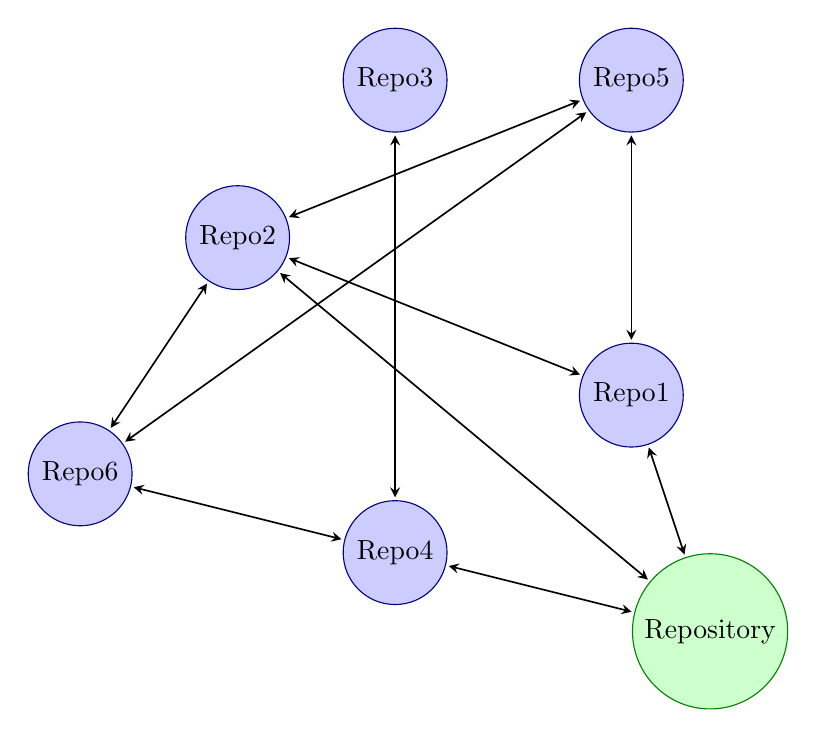
\begin{tikzpicture}
[repo/.style={circle,
		fill=green!20!white,
		draw=green!50!black,
		minimum size=10mm},
workingcopy/.style={circle,
		fill=blue!20!white,
		draw=blue!50!black,
		minimum size=5mm},
link/.style={<->, shorten <=1pt, shorten >=1pt, >=stealth, semithick}]

% working copies
\node at (3,-1)  [workingcopy] (repo1) { Repo1 };
\node at (-2,1)  [workingcopy] (repo2) { Repo2 };
\node at (0,3)   [workingcopy] (repo3) { Repo3 };
\node at (0,-3)  [workingcopy] (repo4) { Repo4 };
\node at (3,3)   [workingcopy] (repo5) { Repo5 };
\node at (-4,-2) [workingcopy] (repo6) { Repo6 };
% links between repos
\draw [link] (repo1) -- (repo2);
\draw [link] (repo1) -- (repo5);
\draw [link] (repo2) -- (repo5);
\draw [link] (repo3) -- (repo4);
\draw [link] (repo6) -- (repo2);
\draw [link] (repo6) -- (repo5);
\draw [link] (repo4) -- (repo6);
% central repo
\node at (4, -4) [repo] (mainrepo) { Repository };
% links to central repo
\draw [link] (mainrepo) -- (repo1);
\draw [link] (mainrepo) -- (repo2);
\draw [link] (mainrepo) -- (repo4);
\end{tikzpicture}

    }
\end{center}

\end{frame}

% vim: expandtab shiftwidth=4:
